\documentclass[UTF8,a4paper]{ctexart}
\usepackage[utf8]{inputenc}
\usepackage{amsmath}
\usepackage{pdfpages}
\usepackage{graphicx}
\usepackage{wrapfig}
\usepackage{listings}
\usepackage{xcolor}
\lstset{
    numbers=left, 
    numberstyle= \tiny, 
    keywordstyle= \color{ blue!70},
    commentstyle= \color{red!50!green!50!blue!50}, 
    frame=shadowbox, % 阴影效果
    rulesepcolor= \color{ red!20!green!20!blue!20} ,
    escapeinside=``, % 英文分号中可写入中文
    xleftmargin=2em,xrightmargin=2em, aboveskip=1em,
    framexleftmargin=2em
} 
\title{模式识别作业6}
\author{张蔚桐\ 2015011493\ 自55}
\begin {document}
\maketitle
\section{}
\subsection{}
首先由分类面形状可以知道(C)图必然为线性核函数得到的结果,同时也可以得到(D)是精细径向基($\sigma=0.1$)得到的结果,(A)是二次多项式核得到的结果。同时,观察支持向量的位置和分类面和线性分类面的差异可以看出,(E)是三次多项式核函数的结果,而(B)是粗糙径向基得到的结果($\sigma=1$),(F)是中等径向基得到的结果($\sigma=0.5$),。总结如下

\begin{table}
\caption{不同分类面对应的核函数}
\centering
\begin{tabular}{|c|c|c|c|}
\hline
a &二次核函数& b &$\sigma=1$径向基 \\
\hline
c &线性核函数& d &$\sigma=0.1$径向基\\
\hline
e &三次核函数& f &$\sigma=0.5$径向基 \\
\hline
\end{tabular}
\end{table}
\subsection{}
观察数据点性质可以看出这些数据点还是可以线性可分的,因此选择线性核函数比较合理,因为比较简单,同时分类效果足够好,又不会产生过拟合情况。
\section{}
选取数字7和9。训练时的正确率和测试时的正确率如下表所示
\begin{table}
\caption{不同分类面对应的核函数}
\centering
\begin{tabular}{|c|c|c|}
\hline
核函数种类&训练时正确率&测试时正确率\\
\hline
线性核函数&96.2\%&95.34\%\\
\hline
二次核函数&98.2\%&0.6681\%\\
\hline
三次核函数&98.6\%&0.5773\%\\
\hline
精细径向基&51.2\%&0.5047\%\\
\hline
中等径向基&97.7\%&0.5047\%\\
\hline
粗糙径向基&96.2\%&0.5047\%\\
\hline
\end{tabular}
\end{table}

结果比较

经过重新训练神经网络模型,Logistic Regression,贝叶斯以及支持向量模型可以看出,神经网络模型的准确度优于其余三种模型,而其余三种模型在支持向量机采用线性核函数的时候基本相同,均在96\%上下浮动,而神经网络模型可以达到98\%以上

神经网络模型的混淆矩阵附加如图\ref{NN},\ref{TNN}所示

\begin{figure}
\centering 
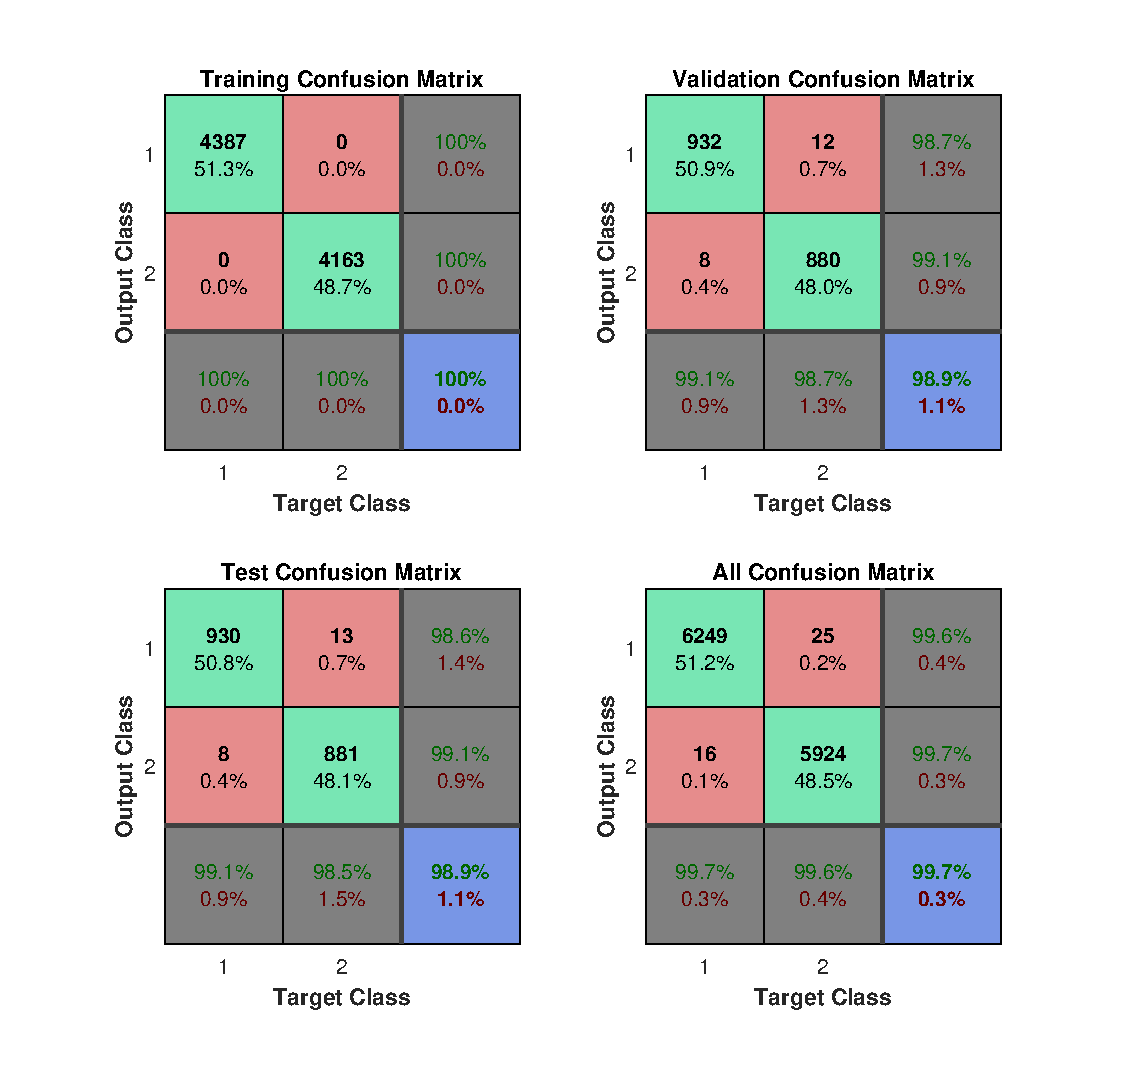
\includegraphics[width=\textwidth]{NNconfi.eps}
\caption{神经网络在训练集上的混淆矩阵}
\label{NN}
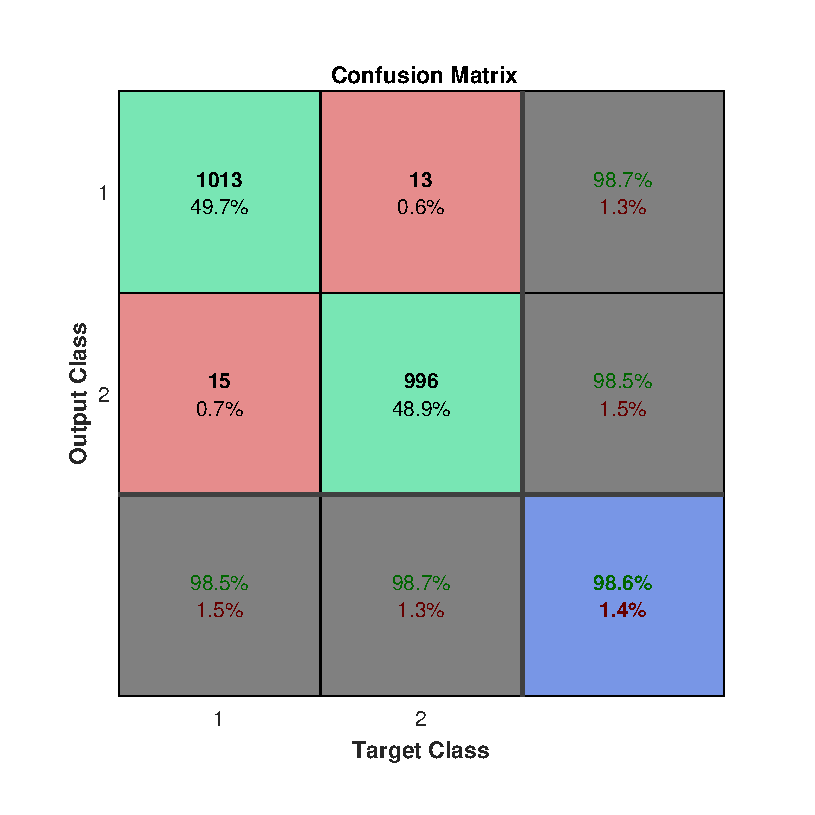
\includegraphics[width=\textwidth]{NNTconfu.eps}
\caption{神经网络在测试集上的混淆矩阵}
\label{TNN}
\end{figure}
\end{document}